\let\negmedspace\undefined
\let\negthickspace\undefined
\documentclass[journal]{IEEEtran}
\usepackage[a4paper, margin=10mm, onecolumn]{geometry}
%\usepackage{lmodern} % Ensure lmodern is loaded for pdflatex
\usepackage{tfrupee} % Include tfrupee package

\setlength{\headheight}{1cm} % Set the height of the header box
\setlength{\headsep}{0mm}  % Set the distance between the header box and the top of the text

\usepackage{gvv-book}
\usepackage{gvv}
\usepackage{cite}
\usepackage{amsmath,amssymb,amsfonts,amsthm}
\usepackage{algorithmic}
\usepackage{graphicx}
\usepackage{float}
\usepackage{textcomp}
\usepackage{xcolor}
\usepackage{txfonts}
\usepackage{listings}
\usepackage{enumitem}
\usepackage{mathtools}
\usepackage{gensymb}
\usepackage{comment}
\usepackage[breaklinks=true]{hyperref}
\usepackage{tkz-euclide} 
\usepackage{listings}
% \usepackage{gvv}                                        
\def\inputGnumericTable{}                                 
\usepackage[latin1]{inputenc}                                
\usepackage{color}                                            
\usepackage{array}                                            
\usepackage{longtable}                                       
\usepackage{calc}                                             
\usepackage{multirow}                                         
\usepackage{hhline}                                           
\usepackage{ifthen}                                           
\usepackage{lscape}
\usepackage{tikz}
\usetikzlibrary{patterns}

\begin{document}

\bibliographystyle{IEEEtran}
\vspace{3cm}

\title{12.573}
\author{ee25btech11063-vejith}

\maketitle
% \maketitle
% \newpage
% \bigskip
{\let\newpage\relax\maketitle}
\renewcommand{\thefigure}{\theenumi}
\renewcommand{\thetable}{\theenumi}
\setlength{\intextsep}{10pt} % Space between text and floats
\textbf{Question}:\\
$\Vec{a}$,$\Vec{b}$,$\Vec{c}$ are three orthogonal vectors. Given that $\vec{a}$=$\hat{i} + 2\hat{j} + 5\hat{k}$ and $\Vec{b}$=$\hat{i} + 2\hat{j} -\hat{k}$, the vector $\vec{c}$ is parallel to \hspace{2.5cm} \brak{\text{IN } 2019}
\begin{enumerate}[label=(\alph*)]
    \begin{multicols}{4}
        \item $\hat{i} + 2\hat{j} + 3\hat{k}$
        \item $2\hat{i} + \hat{j}$
        \item $2\hat{i} - \hat{j}$
        \item $4\hat{k}$
    \end{multicols}
\end{enumerate}
\textbf{Solution}:\\
Given 
\begin{align}
    \vec{a}=\myvec{1\\2\\5}\\
    \vec{b}=\myvec{1\\2\\-1}\\
    \vec{a}^\top\vec{c}=0\\
    \vec{b}^\top\vec{c}=0
\end{align}
(3) and (4) can be written as
\begin{align}
    \myvec{\vec{a}^\top \\ \vec{b}^\top}\vec{c}=\myvec{0\\0}\\
    \implies \begin{pmatrix}
        1 & 2 & 5\\
        1 & 2 & -1
    \end{pmatrix}\vec{c}=\myvec{0\\0}
\end{align}
Forming the augmented matrix
\begin{align}
    \left(\begin{array}{ccc|c}
        1 & 2 & 5 & 0 \\
        1 & 2 & -1 & 0 
\end{array}\right) &\xleftrightarrow{R_2 \rightarrow R_2- R_1} \left(\begin{array}{ccc|c}
        1 & 2 & 5 & 0 \\
        0 & 0 & -6 & 0 
\end{array}\right)
\end{align}
$\implies$ vector $\vec{c}$ can be written in general as $\vec{c}=\myvec{2k\\-k\\0}$ \brak{\text{for some scalar }k}\\
$\implies$ vector $\vec{c}$ is parallel to $2\hat{i} - \hat{j}$
\begin{figure}
    \centering
    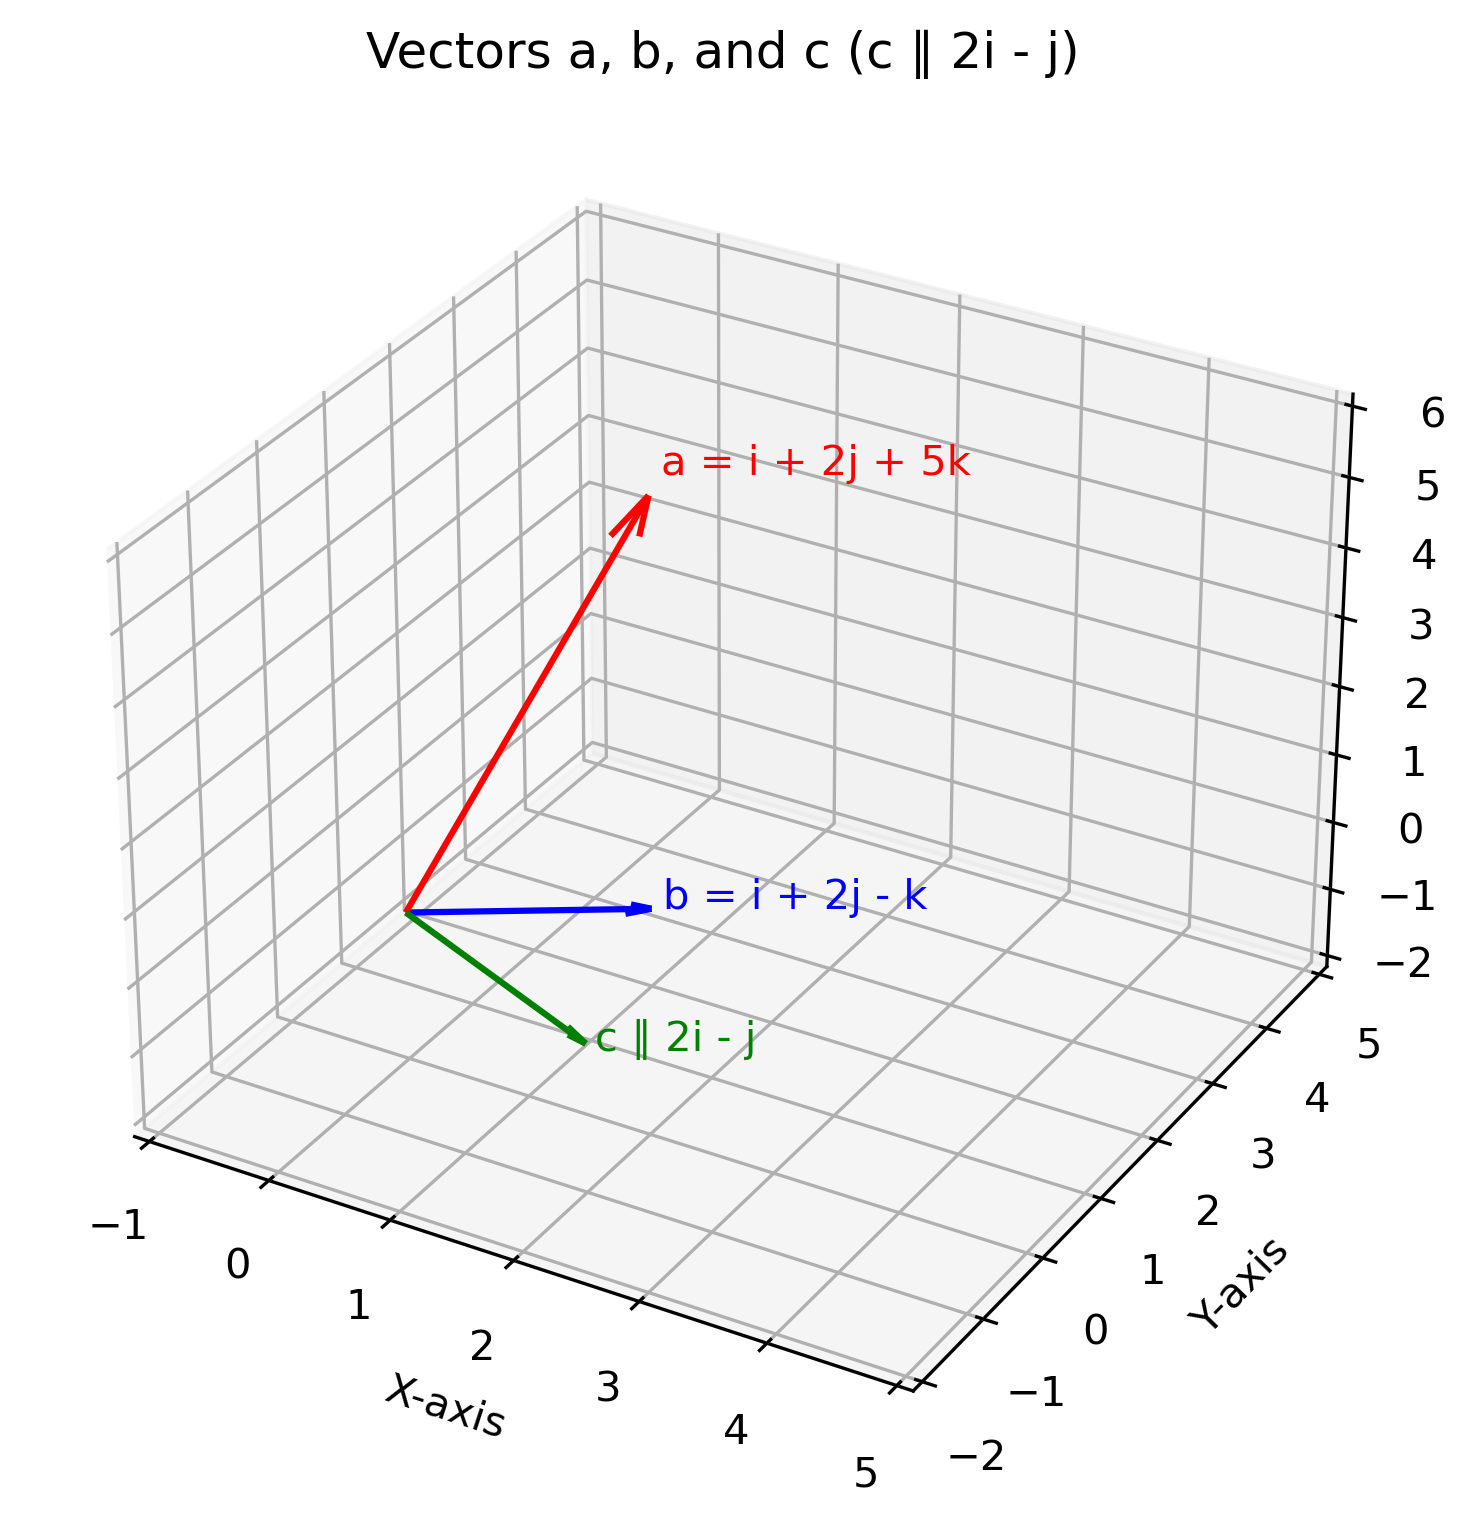
\includegraphics[width=0.52\columnwidth]{figs/01.png}
    \caption{}
    \label{fig:placeholder}
\end{figure}
\end{document}
